%!TEX root = ../../Master.tex
\section{Organisation}
\frnote{Her mangler lidt intro/ meta tekst}

I Aalborg er det kommunen der ejer havnene. Forengninger lejer havnene gratis imod at de selv vedligeholder den. Det er typisk en bådklub pr havn. Ud over det bliver havnene nogle gange benyttet af andre mindre klubber, som kajakklubber eller søspejdere.

Der er 4 store lystbådehavne i Aalborg by:
\begin{itemize}
    \item Marina Fjordpark
    \item Skudehavnen - lystbådehavnsafsnit
    \item Vestre Baadehavn - lystbådehavnsafsnit
    \item Nordre Baadehavn
\end{itemize}

Aalborg kommune har indgået en brugs aftale med Aalborg / Nørresundby Fritidshavn (ANF).

\subsection{Aalborg/Nørresundby Fritidshavn}

ANF er en paraplyorganisation for følgende sejlklubber. \cite{anf_havnereglement}
\begin{itemize}
	\item Aalborg Sejlklub
	\item Fiskerklyngen
	\item Vestre Baadelaug
	\item Sejlklubben Limfjorden
	\item Nørresundby Sejlklub
\end{itemize}
 
 Dette betyder at ANF forestår forhandlinger på vegne af organisationens sejlklubber. En fælles brugsaftale af de fire havne, kan derved indgås med havneejer, Aalborg kommune.

 ANF's indtægter består af bådpladsafgifter, som medlemsklubberne skal betale, for brug af de tilknyttede havne \cite{anf_budget_2013}. ANF forpligter sig til vedligeholdelse af havnene tilknyttet foreningen, herunder hovedistandsættelser samt udføring af nyanlæg \cite{anf_brugsaftale_2012}.

 \begin{figure}
 	\begin{center}
 		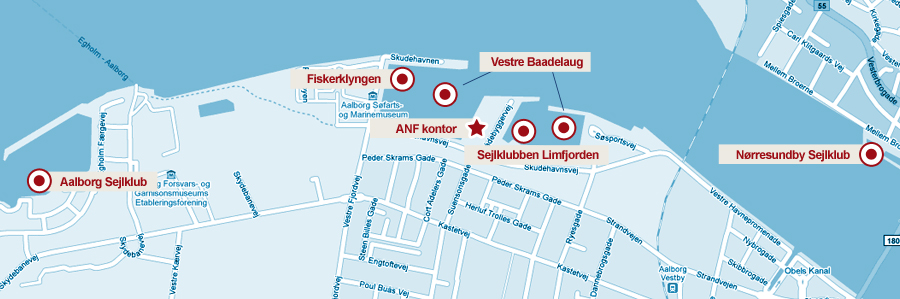
\includegraphics[width=\textwidth]{anf_overblik.jpg}
 	\end{center}
 	\caption{Overblik over medlemmerne af ANF}
 	\label{fig:anf_overblik}
 \end{figure}

\subsection{Bådklubber}
\frnote{vi skal måske havde et afsnit om plads fordeling}
Her vil vi se på de forskellige bådklubber der er med i ANF. Klubberne fordeler deres pladser ud til medlemmerne. Der bliver lave en ny plads fordelig hvert år. Inden den nye pladsfordelig bliver lavet vil det være mulig at ænske om plads til næste år. Der er en masse menneskelige interesser der skal tænkes med når pladsfordelingen skal laves. Det er vigtigt for nogle mennesker hvor de ligger, det er afgørende. Det er ikke mulig at få en permanet plads, men som reglet vil man søge for at et medlem beholder sin plads når fordelingen bliver lavet. Medlemmerne betaler enten pr pladskvadratmeter eller kvadratmeter båd. Et medlem kan kun havde en bådplads, dog kan der opstå situationer hvor et medlem har mere end en båd, bla. i for bidelse med salg \cite{int_vb_sl}.

\subsubsection{Vestre Baadelaug}
Vestre Baadelaug har bådepladser i Vestre Bådehavn og Skudehavnen, som begge deles med Sejlklubben Limfjorden. Klubben har omkring 380 medlemmer \cite{int_vb_sl}. 

\subsection{Sejlkubben Limfjorden}
Sejlkubben Limfjorden har omkring 150 medlemmer \cite{int_vb_sl}. Klubbens medlemmer omfatter kun folk med sejlbåde. Klubben er medlem af Dansk Sejlunion (DS), som er et special forbund under Dansk Idræts Forbund. DS optager klubber i alle former for sejlads som medlemmer. DS har en kollektiv forsikring som medlemsklubberne automatisk er medlem af. 

\subsection{Aalborg Sejlklub}
Aalborg Sejlkulb er en Sejlklub, der høre til i havnen Marina Fjodparken.

\subsection{Nørresundby Sejlklub}
Nørresundby Sejlklub er tilnyttet Nørresundby havn. Klubben er medlem af Dansketur sejlere \cite{norresundby_sejlklub}.

\subsection{Regler og love}
Transportministeriet har i 2002 udgivet en bekendtgørelse om standardreglement for lystbådehavne \cite{standardreglement}. I denne er der regler om hvordan man skal opføre sig når man er på en havn. De enkelte havne skal så udarbejde et individuelt ordensreglement som beskriver hvilket område det gælder for og hvilke særlige ordensregler der skal gælde på havnen. Derudover skal det referere til bekendtgørelsen.

I standardreglementet bliver der talt om hvordan man skal sejle og fortøjer sit fartøj i havnen. Bladt andet står der at gæstende fartøjer skal melder deres ankomst til havnemyndigheden. Og de skal flytte deres fartøj til en anden plads hvis havnemyndigheden siger det. Man har også pligt til jævnligt at holde øje med sit fartøj, når det ligger i havnen. Fartøjet skal være forsvarligt fortøjret og tov skal fastgøres så de ikke klapper mod masten. I reglementet er der regler for optagning, reparation, brændstof og  forskellige miljøbestemmelser.